\chapter{Preparation}
\label{chap:preparation}
After identifying the main goals of the project, these coarse requirements have to be refined, in order to be more precise about my aims and drive the project development.
The result of this is a set of \emph{requirements} that can then be analysed to predict problems and measure success.
Once any problems have been resolved, work can begin on implementation.
Some mathematical theory is also required to state the problem more precisely, and can be used to direct the refinement of requirements.

In this chapter I discuss the background theory required to begin work on the formalisation, briefly introduce my main tool, Isabelle, and produce a list of requirements.

\section{\(\lambda\)-Calculus}
\label{sec:lambda-intro}
The \(\lambda\)-calculus~\cite{lambda-overview} is a formal system of computation represented by operations on an set of terms.
\begin{definition}
Terms \(M\) are inductively defined as follows.
\begin{enumerate}
\item
A variable, \(x\), is always a term.
These may be sub-categorised to be \emph{bound} if some \emph{binder} in an expression binds them, or \emph{free}, if there is no such binder.
\item
If \(M\) is a term, abstractions \(\lambda x.M\) are also terms.
This intuitively represents an anonymous function in the calculus, taking an argument \(x\) and returning \(M(x)\)), and therefore \emph{binds} \(x\) in \(M\).
\item
If \(M\) and \(N\) are terms, applying \(M\) to \(N\) is also a term, \(\wrap{M\ N}\).
\end{enumerate}
\end{definition}

This is straightforward to define programmatically, as it can be represented with an algebraic datatype.
For instance, in Standard ML:
\begin{minted}{SML}
datatype 'a trm =
    Var of 'a
  | Fn  of ('a * 'a trm)
  | App of ('a trm * 'a trm)
\end{minted}

Computation in this system is done by means of \(\beta\)-reduction: terms may \emph{reduce} to another term according to a series of rules, and hence computation occurs by sequential reductions of terms.

\begin{definition}
A term \(M\) \(\beta\)-reduces to \(M'\), \(M \to_\beta M'\) if one of the following holds:
\begin{enumerate}
\item
If the left or right subterms of an application reduce to another term, then the application reduces to the same application with that term reduced.
For instance, if \(M \to_\beta M'\), then \(\wrap{M\ N} \to_\beta \wrap{M'\ N}\).
\item
If the bound term \(M\) of a function reduces to \(M'\), then \(\lambda x.M\) reduces to \(\lambda x.M'\).
\item
If the term is of the form \(\wrap{\wrap{\lambda x.M}\ N}\), then it is a \(\beta\)-redex, and reduces to
\[
M[x := N]
\]
That is, \(M\) with any occurrence of the variable \(x\) substituted in a capture-avoiding fashion for \(N\).
\end{enumerate}
\end{definition}

It turns out that the order in which reduction steps occur in a computation is important for many applications of the \(\lambda\)-calculus, but I did not use this property in any of the results in my dissertation.
Substitution, while used informally above, is itself defined recursively.

\begin{definition}
Suppose \(N\) is substituted for \(x\) in \(M\), and \(y\) is used for any name that is not the same as \(x\).
Then the result, \(M[x := N]\), is defined piecewise as
\[
M[x := N] =
\begin{cases}
N & M = x\\
M & M = y\\
M & M = \lambda x. M'\\
\lambda y. \wrap{M'[x := N]} & M = \lambda y. M'\\
\wrap{M_1[x := N]\  M_2[x := N]} & M = \wrap{M_1\ M_2}\\
\end{cases}
\]
\end{definition}

\(\beta\)-reduction has the notable property of \emph{confluence}, which I show as an extension in the implementation chapter.
Confluence states that if \(A\) reduces in zero or more steps to \(B\), and similarly on a possibly-different path to \(C\), there is a \(D\) such that \(B\) and \(C\) both reduce to \(D\).
This asserts that the order in which reductions are carried out on a term do not affect the final result.
One consequence of reduction is that there are terms that cannot be further reduced: \(x\) is one example, as is \(\lambda y.y\), or \(\wrap{f\ x}\).
These terms are considered to be values, or \emph{in normal form}.

\begin{definition}
Variables \(x\) are in normal form.
Applications are in normal form if they are not a \(\beta\)-redex and both subterms are themselves in normal form.
Binders are in normal form if their bound subterm is in normal form.
\end{definition}

\section{Simple Types}
\label{sec:type-intro}
Untyped calculi have several disadvantages.
A lack of type system means that unexpected or nonsensical constructions can be made (such as applying a non-function), which a type system generally prevents.
``Programs'' encoded in the calculus may also fail to terminate: a sequence of reductions may not necessarily finish.
Consider

\[
\Omega = \wrap{\lambda x. \wrap{x\ x}}\ \wrap{\lambda x. \wrap{x\ x}}
\]

Then the only possible reduction rule for \(\Omega\) produces \(\Omega\) itself, without any possibility of termination.
The untyped calculus can be extended to include a type system without any effect on the theory of names it uses: a \emph{type} is simply added to each binder, so \(\lambda x.M\) becomes \(\lambda (x:T).M\), for an arbitrary \(T\).
Note that this is the Church style of typing, as opposed to the Curry style.
I use this style exclusively in my project.

\begin{definition}
Simple types \(\tau\) are either
\begin{enumerate}
\item
A (fixed) base type, say \(\iota\).
\item
An arrow type \(\tau \to \tau\) from one type to another.
\end{enumerate}
\end{definition}

Adding simple types to the binders of the untyped calculus produces the \emph{simply-typed} \(\lambda\)-calculus.
The typing relation \(\Gamma \vdash M : \tau\) is given inductively in Figure \ref{fig:typing}.
\(\Gamma\) here is a typing context: a partial function from variables to types.

\begin{figure}
\begin{mathpar}
\inferrule[var]
 {\Gamma(x) = \tau}
 {\Gamma \vdash x : \tau}

\inferrule[fn]
 {\Gamma\{x \mapsto \tau\} \vdash M : \sigma}
 {\Gamma \vdash \lambda (x : \tau). M : \tau \to \sigma}

\inferrule[app]
 {\Gamma \vdash M : \tau \to \sigma \\ \Gamma \vdash N : \tau}
 {\Gamma \vdash \wrap{M\ N} : \sigma}
\end{mathpar}
\caption{typing rules for the simply-typed calculus}
\label{fig:typing}
\end{figure}

Using these typing rules, I show several correctness properties in my implementation that are not possible in an untyped calculus: progress, type preservation (also known as subject reduction), and safety.
These capture several possible meanings behind the Milner's~\cite{milner} maxim ``well-typed programs do not go wrong''.

\begin{definition}
The progress property states that if a term is well-typed, then it is either in normal form or can be reduced further.
\end{definition}

\begin{definition}
The preservation property holds if, when a term has a given type \(\tau\), it still has the same type after being reduced.
\end{definition}

Generally these are desirable properties in a language: expressions should not ``get stuck'' computing non-values, or change type mid-reduction (for example, reducing from an integer-typed expression to a string).

\begin{definition}
A language has the safety property if reducing a well-typed term by an arbitrary number of steps results in another term that is either in normal form, or can be reduced further.
\end{definition}

This property is the main aim of the verification: it shows that if a term is well-typed, then there is no scenario in which reduction can fail --- either the term keeps reducing, or the computation has finished.

Type inference is the process of producing a type \(\tau\) for term \(M\) such that \(M\) has this type under some \(\Gamma\).
One advantage of the simply-typed calculus is that type inference is a straightforward algorithm, with no unification steps (at least in the Church style) or other complexity that comes with more advanced typing systems.
A type inference algorithm \(\infertype(\Gamma, M)\) can be described recursively by
\[
\infertype\wrap{\Gamma, M} =
\begin{cases}
\Gamma(x) & M = x\\
\tau \to \infertype\wrap{\Gamma\{x \mapsto \tau\}, N} & M = \lambda (x : \tau). N\\
\mathrm{apply}\wrap{\infertype\wrap{\Gamma, A}, \infertype\wrap{\Gamma, B}} & M = \wrap{A\ B}
\end{cases}
\]
where \(\mathrm{apply}\wrap{\tau \to \sigma, \tau}\) produces \(\sigma\) for any \(\tau, \sigma\), and all other input is undefined.
In my implementation, I use an option type to recognise failure and propagate errors up to the top of the stack, but the presentation above omits this for simplicity.
Type inference can be shown to be correct with respect to a type system if it only infers correct types (it is \emph{sound}) and infers all types that are valid typing judgements (it is \emph{complete}).
Then the two are equivalent, and any property the typing system has, the type inference algorithm also has.

\section{The Problem of \(\alpha\)-Equivalence}
\label{sec:alpha-equivalence}
Unfortunately, this representation with names and binders has a problem: frequently, it is convenient to reason that e.g. \(\lambda x.x\) and \(\lambda y.y\) are the same: they do, after all, compute equal values on all inputs.
However, structurally-speaking they are not equal: the string \(x\) is not the same as \(y\).
This reasoning principle is called \emph{\(\alpha\)-equivalence}.

\begin{definition}
The \(\alpha\)-equivalence relation \(\equiv_\alpha\) is the least congruence on terms such that
\[
\lambda x.M \equiv_\alpha \lambda y.M'
\]
where y does not occur free in \(M\), and \(M'\) is \(M\) with \(x\) substituted for \(y\) in a capture-avoiding fashion.
\end{definition}

Such a definition can be implemented in a proof assistant, then used whenever a statement of equivalence is required.
It also conveniently forms an equivalence relation.
It is nonetheless rather cumbersome and inefficient to carry such an assumption around, and proof assistants often reason better about actual equality than arbitrary equivalence relations, as automation tools tend to be optimised for equality.
This problem can be solved by using \emph{quotient types}~\cite{quotient}.

\begin{definition}
A quotient type \(Q\) consists of a base type \(R\), an equivalence relation \(\sim\) on \(R\), and functions \(\mathrm{Abs} : R \to Q\) and \(\mathrm{Rep} : Q \to R\).
Items \(q_1 : Q\) and \(q_2 : Q\) are equal iff \(Rep\ q_1 \sim Rep\ q_2\).
\end{definition}

I use this operation to define a type for \(\lambda\)-terms modulo \(\alpha\)-equivalence by encoding a datatype for pre-terms without a notion of equivalence as before, then producing the new type as a quotient type over the \(\alpha\)-equivalence relation.

While we can now use equality directly instead of an equivalence relation, the definition of the equivalence relation is quite awkward to use.
There are several alternative ways of handling names and \(\alpha\)-equivalence, the most prominent being de Bruijn indices~\cite{deBruijn}, Higher-Order Abstract Syntax~\cite{HOAS} (or HOAS for short), and nominal techniques~\cite{nominal}.
Ideally, these representations would allow the ``Barendregt convention'' for reasoning about names: for any given term, one may assume that the bound variables are distinct from each other, and from any free variables in the term~\cite{lambda-overview}.
This simplifies proofs about name-carrying syntax, and is widely useful in informal reasoning about \(\lambda\)-calculus.

De Bruijn indices remove names altogether and instead uses natural numbers for bound variables to refer to the number of binders between the variable and the binder that bound it.
For instance, the constant function
\[
\lambda x. \lambda y. x
\]
becomes
\[
\lambda.\lambda. 1
\]
using de Bruijn indices.
Using this approach, \(\alpha\)-equivalence is now simply equality, as all bound names have been removed.
The downside of this approach is that actually using this representation for proofs is quite difficult and unintuitive.
There are several variations on this, including de Bruijn levels (counting binders relative to the start of the term, not relative to the variable --- the constant function becomes \(\lambda.\lambda. 0\)), and several conventions separating free names and bound variables~\cite{i-am-a-free-variable} syntactically, but the main disadvantage is still the same: reasoning is complicated by arithmetic manipulation.

Higher-Order Abstract Syntax uses the environment's (in this case Isabelle's) own binder implementation (i.e. what it uses internally for its own function objects) to handle binding.
The datatype defined earlier for the calculus would then be implemented as
\begin{minted}{SML}
datatype trm =
    Fn  of (trm -> trm)
  | App of (trm * trm)
\end{minted}
The constant function would be represented as \mintinline{SML}{Fn (fn x => Fn (fn y => x))}.
While this implementation neatly avoids many of the implementation issues of other approaches, it is not always possible to show certain properties of names with this representation~\cite{HOAS}.
Manipulating terms also becomes counter-intuitive, as functions have to be un-wrapped and re-wrapped to access the terms under them.
Additionally, this representation is not strictly-positive, so cannot be represented in many proof assistants, which requires positive datatypes to avoid inconsistencies~\cite{inductive-types}.
Another theoretical issue arises from the ability of users to place arbitrary terms in the host language under binders, some of which may not be term constructors, so the representation is too permissive, allowing encoding of ``junk terms''.

Parametric HOAS~\cite{PHOAS} reduces some of these problems by re-introducing a variable constructor and parameterising binders over a set of variables, not over terms.
The representation is then more like the following, reducing the effect of arbitrary exotic terms (since users can only write functions depending on an opaque type of variables), and the datatype is now strictly-positive:

\begin{minted}{SML}
datatype 'var trm =
    Var of 'var
  | Fn of ('var -> 'var trm)
  | App of ('var trm * 'var trm)
\end{minted}

Finally, the ideas under the heading of ``nominal techniques''~\cite{nominal} introduced by Gabbay and Pitts are a relatively-new approach of dealing with names, which importantly retain the explicit representation of names, as in the na\"ive version above.
The technique uses a different definition of \(\alpha\)-equivalence based on \emph{permuting} (rather than substituting) names in a given expression.
This was the approach that I chose, as it allowed an intuitive representation of the calculus, without compromising on usability or theoretical properties, but still allowing concise arguments.

Several further techniques exist, including some very recent research into viewing \(\lambda\)-terms as maps of occurrences of variables in a syntactic tree~\cite{term-maps}, so this is still an active research area, with new approaches in continuous development.

\section{Nominal Techniques}
\label{sec:nominal-intro}
I use the following, simplified presentation of the nominal idea of \(\alpha\)-equivalence in my project, but the theoretical background is much more involved and general.
I present the simplified idea first, then an overview of the generality of nominal techniques.

\begin{definition}
A swapping \([x \swap y]\) is a pair of variables \(x\), \(y\).
\end{definition}

These represent the action of changing instances of \(x\) to \(y\) and \(y\) to \(x\) within a structure, leaving other variables unchanged.

\begin{definition}
The effect of a swapping on a term, \([x \swap y] \cdot M\) is defined as
\[
[x \swap y] \cdot M =
\begin{cases}
y & M = x\\
x & M = y\\
z & M = z, z \notin \{x, y\}\\
\lambda ([x \swap y] \cdot z). \wrap{[x \swap y] \cdot N} & M = \lambda z.N\\
\wrap{[x \swap y] \cdot A}\ \wrap{[x \swap y] \cdot B} & M = \wrap{A\ B}
\end{cases}
\]
\end{definition}
An equivalence \(\sim\) can be defined using only this operation, as shown in Figure \ref{fig:nominal}.
\begin{figure}
\begin{mathpar}
\inferrule[var]
 { }
 {x \sim x}

\inferrule[app]
 {A \sim C \\ B \sim D}
 {\wrap{A\ B} \sim \wrap{C\ D}}

\inferrule[fn]
 {[z \swap x] \cdot M \sim [z \swap y] \cdot N \\ z \# M \\ z \# N}
 {\lambda x.M \sim \lambda y.N}
\end{mathpar}
\caption{an equivalence defined in terms of swappings}
\label{fig:nominal}
\end{figure}
It can further be shown~\cite{nominal-binders} that \(\sim\) is precisely the same as \(\equiv_\alpha\), and hence can be used in place of it.

Therefore my strategy for representing terms modulo \(\alpha\)-equivalence will be to develop a theory of swappings, then use it to argue that \(\sim\) is an equivalence relation, and finally produce a new type as a quotient of the concrete type with respect to \(\sim\).

Looking at the \textsc{Fn} rule of Figure \ref{fig:nominal}, the preconditions \(z \# M\) and \(z \# N\) merit explanation: \(x \# M\) is the statement ``x is \emph{fresh} for M''.

\begin{definition}
An element \(x\) is fresh in a set \(S\) iff \(x \notin S\).
Moreover, a variable \(x\) is fresh for a term \(M\) iff \(x\) is fresh for the free variables of \(M\).
\end{definition}

The idea of picking a fresh item for a given set is common in proofs about the nominal approach to binding.
As a result, I also need a verified implementation of freshness to argue neatly about binding in Isabelle.

\begin{center}
\rule{.3\textwidth}{.5pt}
\end{center}

\noindent
These definitions will suffice for my project.
However, they are a particular instantiation of a more general theory, presented briefly here and in more detail elsewhere~\cite{nominal,nominal-talk,gabbay}.

Consider a set \(\names\) of \emph{names}.
Then, there is another set \(\textrm{Perm}(\names)\), which is the set of finite permutations on \(\names\).
This set forms a group: the group operator is composition, and identity is the identity permutation \(\varepsilon\).
Each permutation has an inverse.
Note here that every permutation can be decomposed into a sequence of swappings, permutations which only swap two variables, and hence composition is simply appending lists of swappings.

The \emph{action} of a permutation \(\pi\) on a set \(X\) which contains \(\names\) in its structure --- for instance, the set of \(\lambda\)-terms using \(\names\) as variables --- maps \(X\) onto itself, intuitively ``permuting the names in \(X\)''.
\begin{definition}
The action of \(\pi\) on \(X\), \(\pi \cdot X\), is a function that satisfies \(\pi_1 \cdot \pi_2 \cdot x = \wrap{\pi_1 \circ \pi_2} \cdot x\), and is the identity function when \(\pi\) is the identity permutation.
\end{definition}

If \(x\) is in such a set \(X\), some set of names may \emph{support} it: if a permutation does not change these names, the permutation action will not change \(x\).
In the \(\lambda\)-calculus under \(\alpha\)-equivalence, these support names are the free variables of \(x\), as permuting bound variables will not change the term under \(\alpha\)-equivalence, but changing free variables does change \(x\).
The freshness relation is then defined more generally in terms of the support of a term.

\begin{definition}
A set \(X\) is a nominal set if for each \(x \in X\) there is a finite set of names that supports \(x\).
\end{definition}

Nominal sets form a category, where objects are nominal sets, and arrows are \emph{equivariant} functions, functions \(f\) that form a commutative diagram with any permutation \(\pi\), as shown in Figure \ref{fig:equivariant}.

\begin{figure}
\[
\begin{CD}
X	@>\pi>>	X\\
@VVfV		@VVfV\\
Y	@>\pi>>	Y
\end{CD}
\]
\caption{A commutative diagram showing the behaviour of an equivariant function.}
\label{fig:equivariant}
\end{figure}

Each nominal set \(X\) yields another nominal set \([\names]X\), where the inhabitants are \emph{name-abstractions} \(\langle a \rangle x\), equipped with an equivalence relation \(\sim\).
\(\langle a \rangle x \sim \langle b \rangle y\) iff there is a new name \(c\), fresh for \(a, b, x, y\) such that \([a \swap c] \cdot x = [b \swap c] \cdot y\).
The permutation action on \([\names]X\) is defined to be such that \(\pi \cdot \wrap{\langle a \rangle x} = \langle \pi \cdot a \rangle\wrap{\pi \cdot x}\).
By using this definition with the special case of \(\lambda\)-terms, Gabbay arrives at the definition presented in Figure \ref{fig:nominal}.

\section{Isabelle}
\label{sec:isabelle-intro}
Isabelle~\cite{isabelle} is a logical framework, supporting several separate object logics (although I use Higher-Order Logic, the default), a number of automated theorem provers and other proof methods to remove tedious proof steps, and a human-readable proof script language, Isar~\cite{isar-phd}.
Proofs are created and checked in Isabelle by providing any definitions (functions, datatypes, inductive definitions, abbreviations) you wish to make, then arguing any theorems you wish to prove in the context of these definitions.
Since each step is checked, the theorems must be logically correct with respect to the definitions used.
There are also a variety of other useful features that Isabelle provides that I use in my project.

Quotient types are used heavily in my dissertation, both for equivalence of permutations (introduced later to implement the nominal approach more easily), and for \(\alpha\)-equivalence.
Isabelle provides this mechanism via a \texttt{quotient\_datatype} command~\cite{isabelle-quotient}, which takes a base type \(R\) and an equivalence relation \(\sim\) and produces a new quotient type \(Q\), \(\mathrm{Abs}\) and \(\mathrm{Rep}\).
It also provides ``lifting'' and ``transfer'' operations, useful for lifting operations from the base type to the quotient type, and transferring proof obligations from the quotient type to the base type.
Type classes~\cite{isabelle-typeclasses} are another Isabelle feature that I used.
They provide a way for types to conform to an interface (for instance, all types that can be ordered might form an ordering typeclass), which I used to implement freshness parametrically on any type.

A major advantage of Isabelle over other proof software was the straightforward support for quotient types.
Isabelle's type-theoretic rivals Agda and Coq both suffer from ``setoid hell'', in which non-equality equivalence relations must be passed around to reason about propositions involving equivalence.
There is no direct equivalent of \texttt{quotient\_type}, and the theory becomes somewhat involved to implement such a construct~\cite{quotients-hard}.
Isabelle also has excellent tooling and a stable core, and these factors combined made it a good choice for my project.

\section{Requirements Analysis and Engineering}
\label{sec:requirements}
Moving from coarse requirements to finer ones is now more straightforward, as a number of constraints have been imposed by the mathematics.
Implementation in Isabelle can then be broken into the following steps:
\begin{enumerate}
\item
Develop formalised work about freshness and swappings to support later developments.
\item
Define a datatype for representing simple types.
\item
Define the datatype of \emph{pre-terms}, the type of terms before the \(\alpha\)-equivalence quotient.
\item
Define the effect of swappings on pre-terms.
\item
Define the \(\alpha\)-equivalence relation
\item
Prove sufficent lemmas to show it is an equivalence relation.
\item
Define a type inference algorithm on pre-terms and show that it is invariant under \(\alpha\)-equivalence.
\item
Produce a quotient type of \emph{terms} from the pre-terms and the equivalence relation.
\item
Lift any required definitions over the quotient, along with the type inference algorithm.
\item
Prove any required lemmas by reference to the same lemmas upon pre-terms.
\item
Define a typing relation inductively on the terms.
\item
Argue properties of this typing relation, such as the subject reduction property.
\item
Show that the inference algorithm is sound and complete with respect to the typing relation.
\item
Conclude that the implementation is verified and extract code.
\end{enumerate}

The dependencies between these steps are largely sequential, as shown in the dependency graph in Figure \ref{fig:requirements-dependencies}.
Additionally, each step could only be ``complete'', or ``incomplete'', considering the boolean nature of formal verification development.
With this in mind, a waterfall model of development seemed appropriate: any topological sort of the dependency graph would suffice to follow such a model.
However, Isabelle allows admitting propositions as axioms, so to a limited extent proofs can follow an iterative model where the number of steps in a proof is progressively made more explicit, with fewer admitted steps.

\begin{figure}
\centering
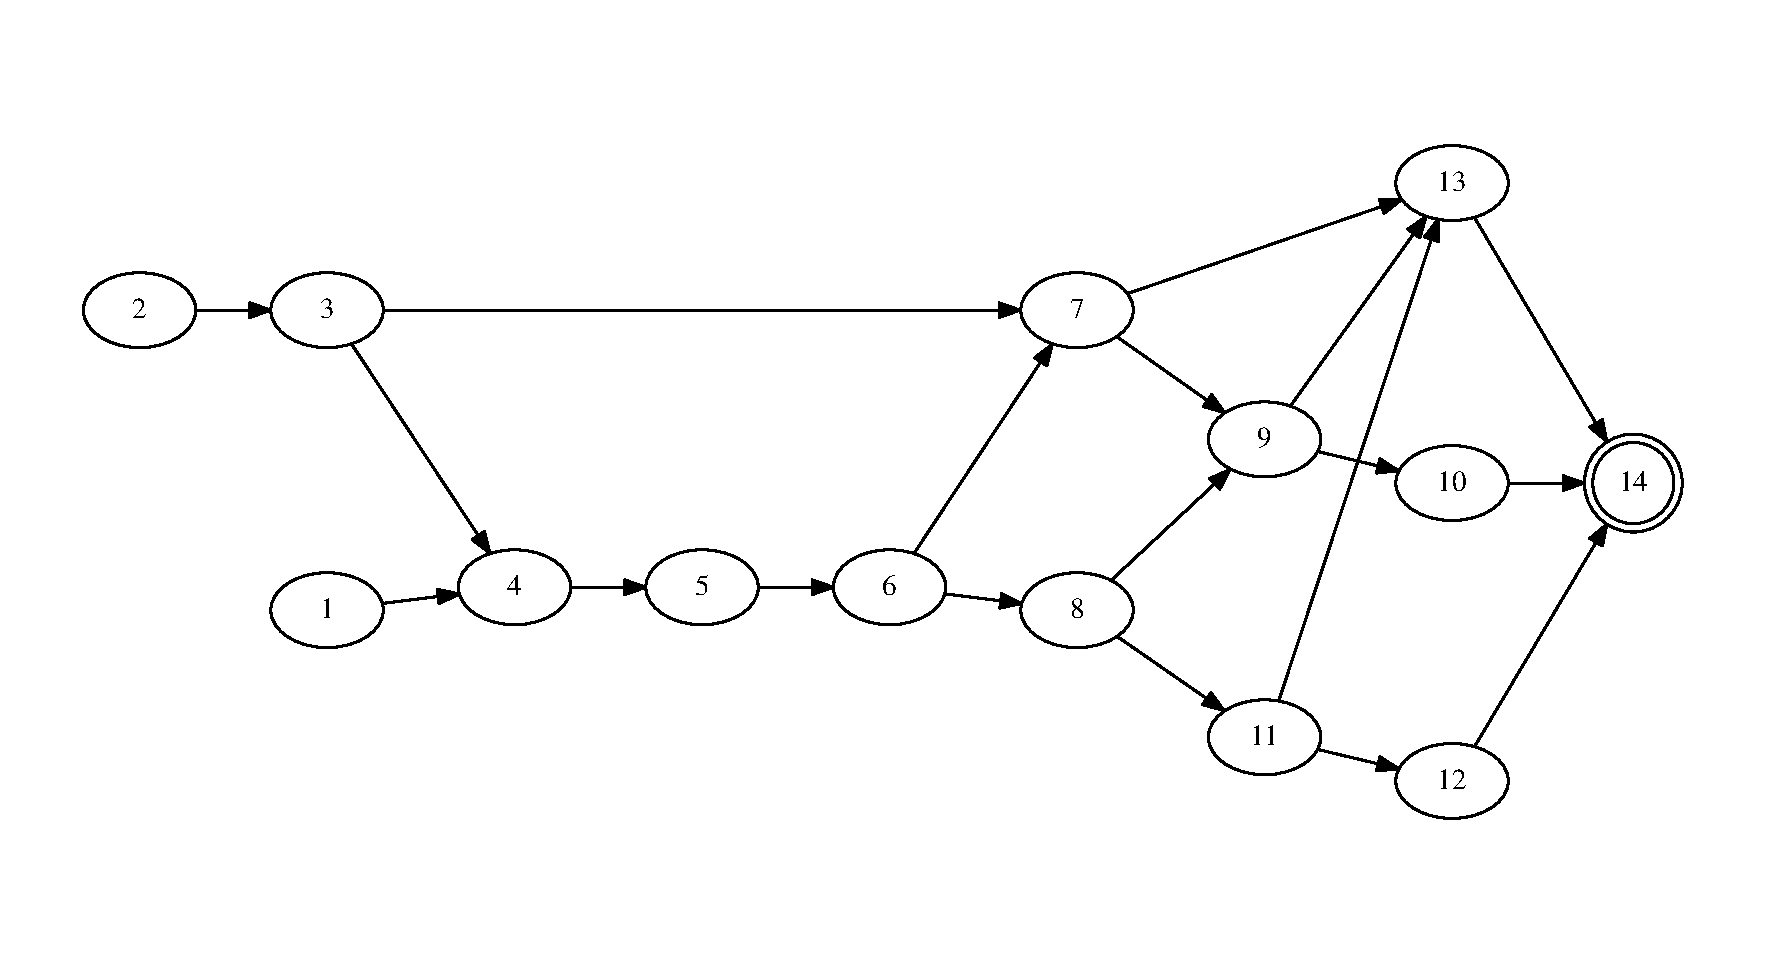
\includegraphics[width=\textwidth]{chapters/preparation/figures/dependencies}
\caption{A directed graph showing which tasks must be completed to begin others. \(A \to B\) shows that \(A\) must be complete before \(B\) may begin.}
\label{fig:requirements-dependencies}
\end{figure}

As far as possible, I followed good software engineering practices with this project.
All project files were checked into version control software (git), and shared (read-only) with supervisors using the GitHub version control platform.
Weekly progress meetings were observed to ensure the project did not get off-track.

\section{Starting Point}
As stated in my original project proposal, I was familiar with the majority of the theory required for implementing the \(\lambda\)-calculus and type theory in the project.
I was not familiar with the number of approaches to handling name binding described above, or with Isabelle itself.
I am pleased to say that I have now learned a lot more about both of these topics.

\section{Summary}
In this chapter I discussed work that took place before starting to implement the project.
I introduced the theoretical background of the project, covering the untyped \(\lambda\)-calculus (\S\ref{sec:lambda-intro}), simple types (\S\ref{sec:type-intro}), \(\alpha\)-equivalence and several approaches to this problem (\S\ref{sec:alpha-equivalence}), and a short introduction to nominal techniques (\S\ref{sec:nominal-intro}), as developed by Gabbay and Pitts \emph{et al}.
I then introduced the Isabelle tooling used in the project (\S\ref{sec:isabelle-intro}), preparing for both practical and theoretical issues in the implementation phase.
Finally, I broke the project down into manageable steps (\S\ref{sec:requirements}), and briefly described engineering techniques used to tackle the problem.
